\documentclass[11pt,a4paper]{article}

\usepackage[margin=1in]{geometry}
\usepackage{graphicx}
\graphicspath{{../figures/}}
\usepackage{amsmath,amssymb}
\usepackage{booktabs}
\usepackage{hyperref}
\usepackage{xcolor}
\usepackage{caption}
\usepackage{tabularx}

\hypersetup{
    colorlinks=true,
    linkcolor=blue!60!black,
    urlcolor=blue!60!black,
    citecolor=blue!60!black,
    pdftitle={ENGR 78 Final Project Report: PlutoSDR Modulation Visualizer},
    pdfauthor={Howard Wang, Kaw Moo, Charlie Schuzte},
    pdfsubject={Final Project Report}
}

\title{\textbf{Real-Time Digital Modulation and Channel Impairments\\with a Single ADALM-PLUTO SDR}\\[0.4em]
\large ENGR 78 --- Final Project Report}
\author{Howard Wang \and Kaw Moo \and Charlie Schuzte}
\date{Spring 2026}

\begin{document}
\maketitle

\begin{abstract}
\noindent
We built a Python app that sends and receives a modulated signal on one ADALM-PLUTO in loopback, adds software channel impairments, and shows spectrum, constellation, eye diagram, BER/EVM/SNR, and throughput in real time. The receiver uses a Barker preamble, frequency/phase estimation, and Gardner timing recovery. A second mode sweeps SNR and plots BER against theory for BPSK, QPSK, 8-PSK, and 16-QAM. Code and this report are on GitHub (link below).
\end{abstract}

\section{What we built}
The goal was a hands-on way to see how noise, phase/frequency offset, multipath, and fading affect a link---without needing two radios. One PlutoSDR in TX--RX loopback plus software impairments does the job.

\noindent\textbf{Features:} Gray-coded BPSK/QPSK/8-PSK/16-QAM with RRC pulse shaping ($\alpha=0.35$, 8 sps); Pluto or software loopback; sliders for AWGN, phase, frequency offset, multipath, and Rician fading; live plots + BER sweep with theory curves.

\begin{figure}[htbp]
    \centering
    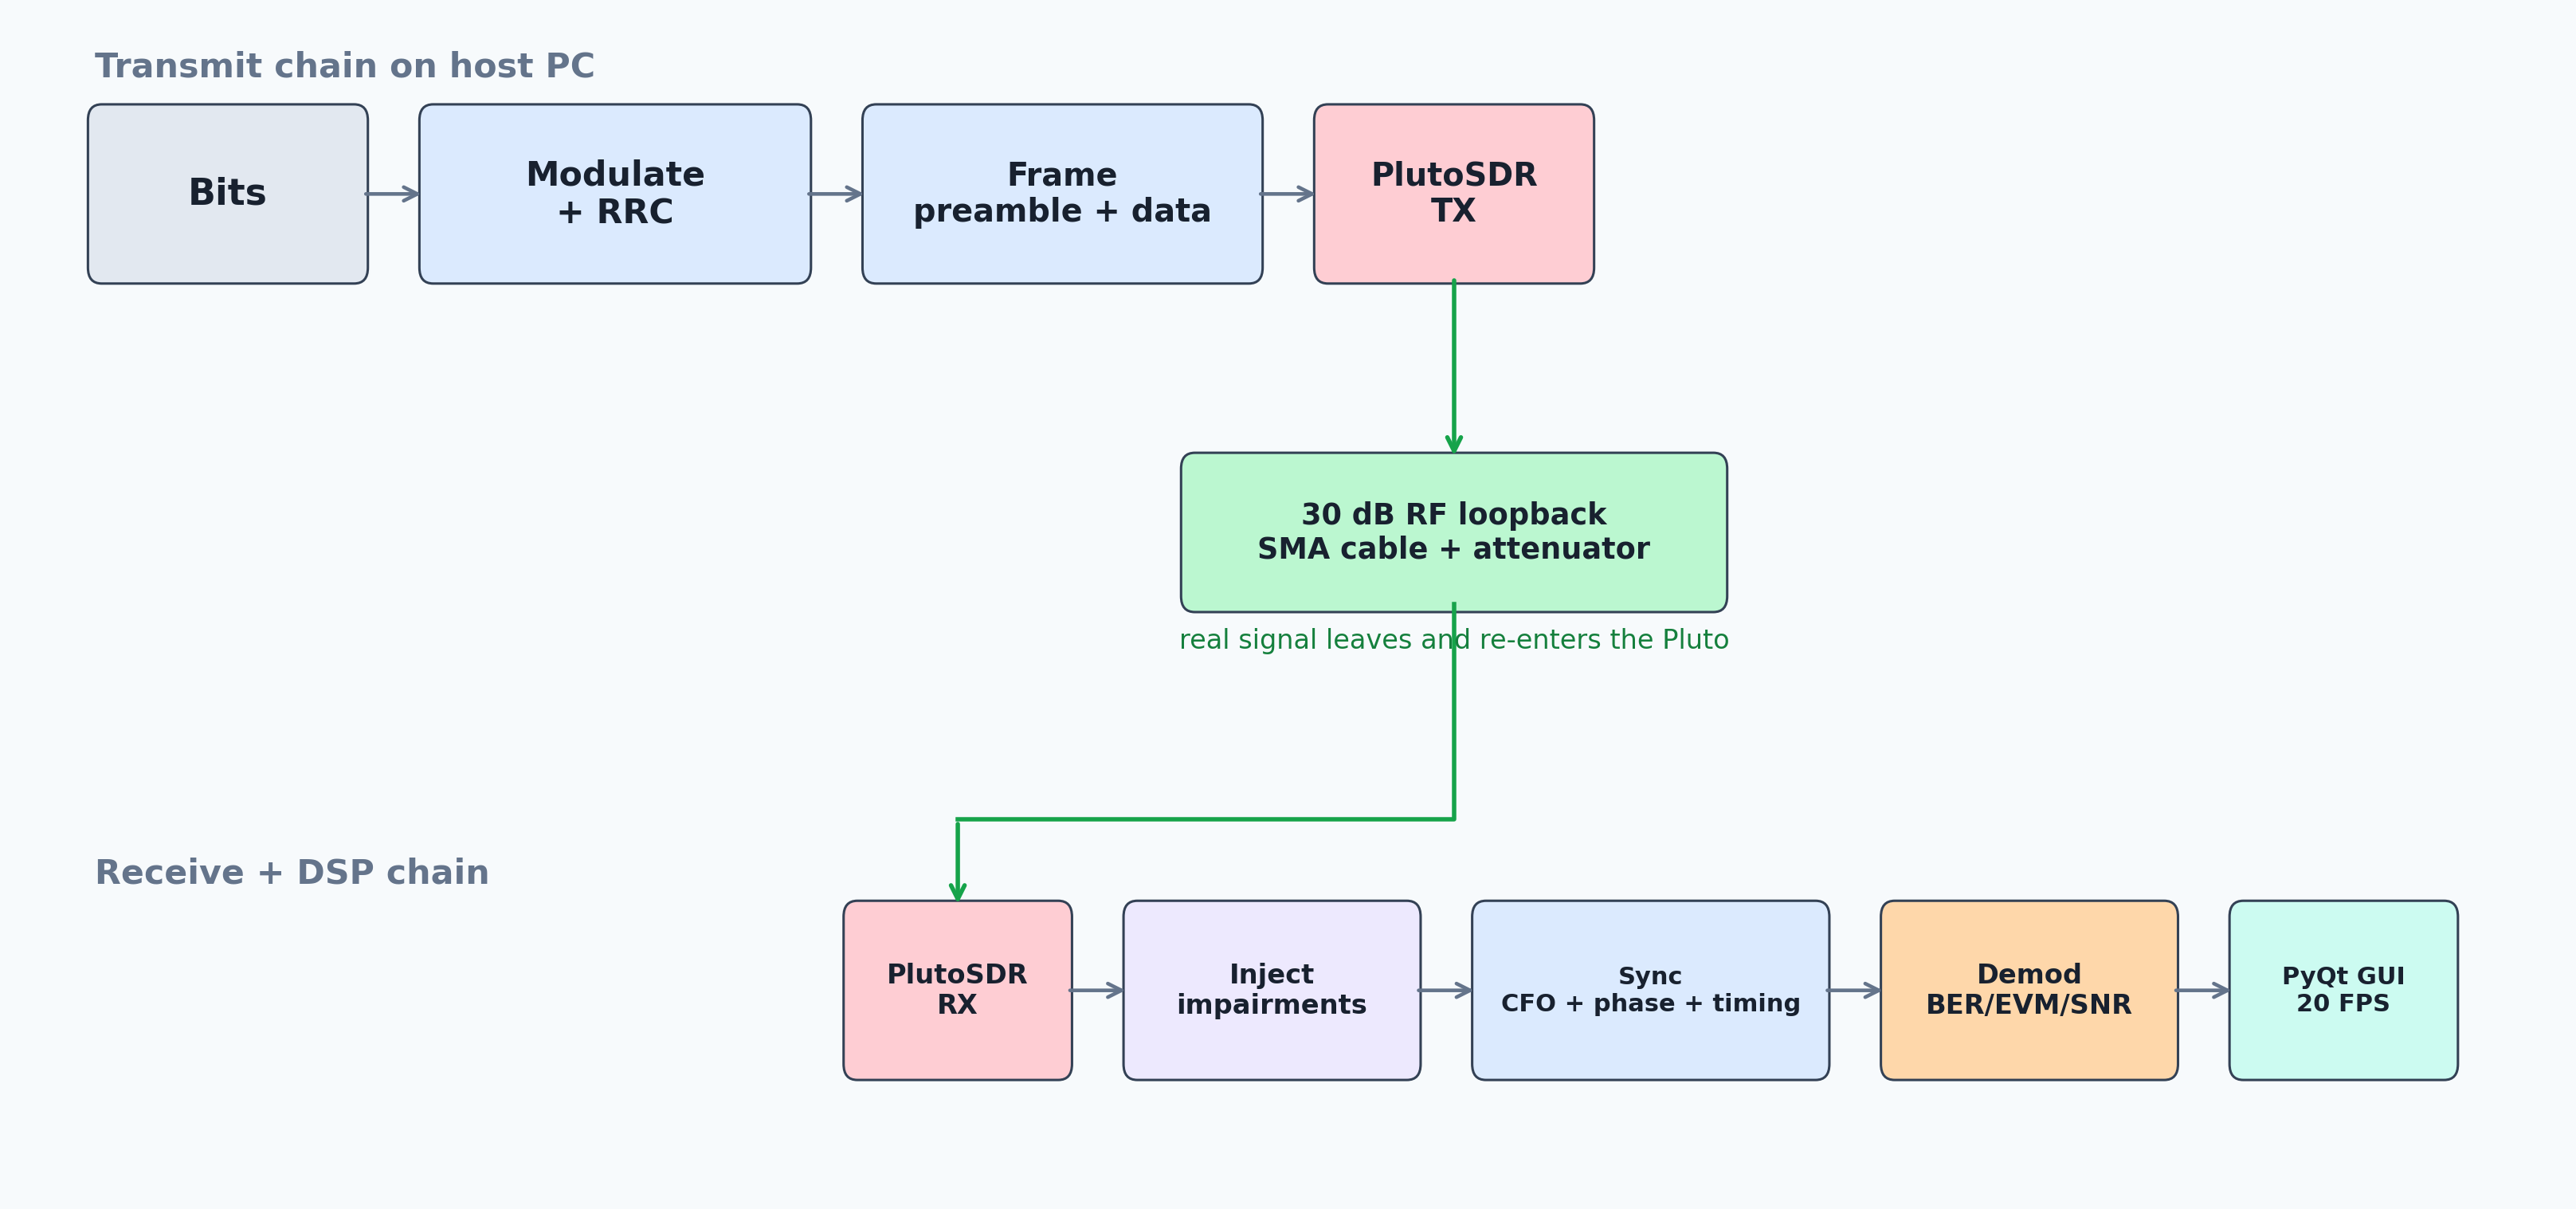
\includegraphics[width=0.95\textwidth]{block_diagram_v2.png}
    \caption{Signal flow: TX, RF loopback, impairments after RX, sync and demod, GUI.}
    \label{fig:block}
\end{figure}

\noindent\textbf{Hardware:} TX to RX with SMA cable, \textbf{30~dB attenuator} before RX, USB to PC. No Pluto? Use simulation mode---same DSP and GUI.

\section{Background (short)}
Symbols are pulse-shaped and demodulated with a matched filter and hard decisions. Impairments are applied in fixed order: multipath $\rightarrow$ fading $\rightarrow$ frequency offset $\rightarrow$ phase offset $\rightarrow$ AWGN (see Figure~\ref{fig:chain}). The receiver finds the frame via preamble correlation, estimates CFO and phase, and tracks timing with a Gardner loop.

\begin{figure}[htbp]
    \centering
    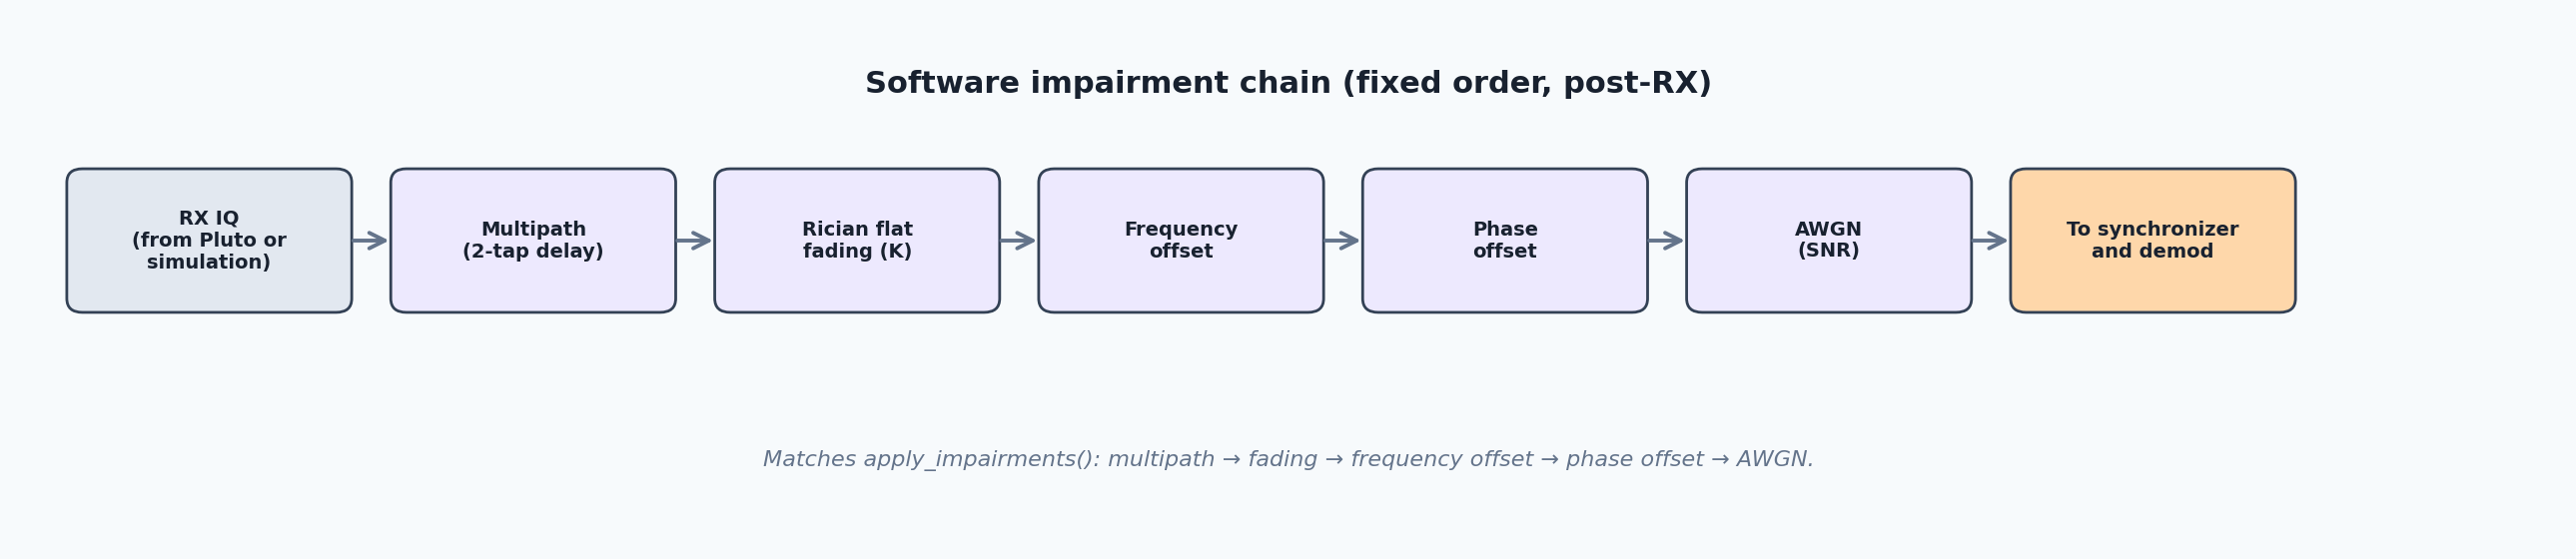
\includegraphics[width=\textwidth]{impairment_chain.png}
    \caption{Impairment order in software (matches \texttt{apply\_impairments}).}
    \label{fig:chain}
\end{figure}

\begin{figure}[htbp]
    \centering
    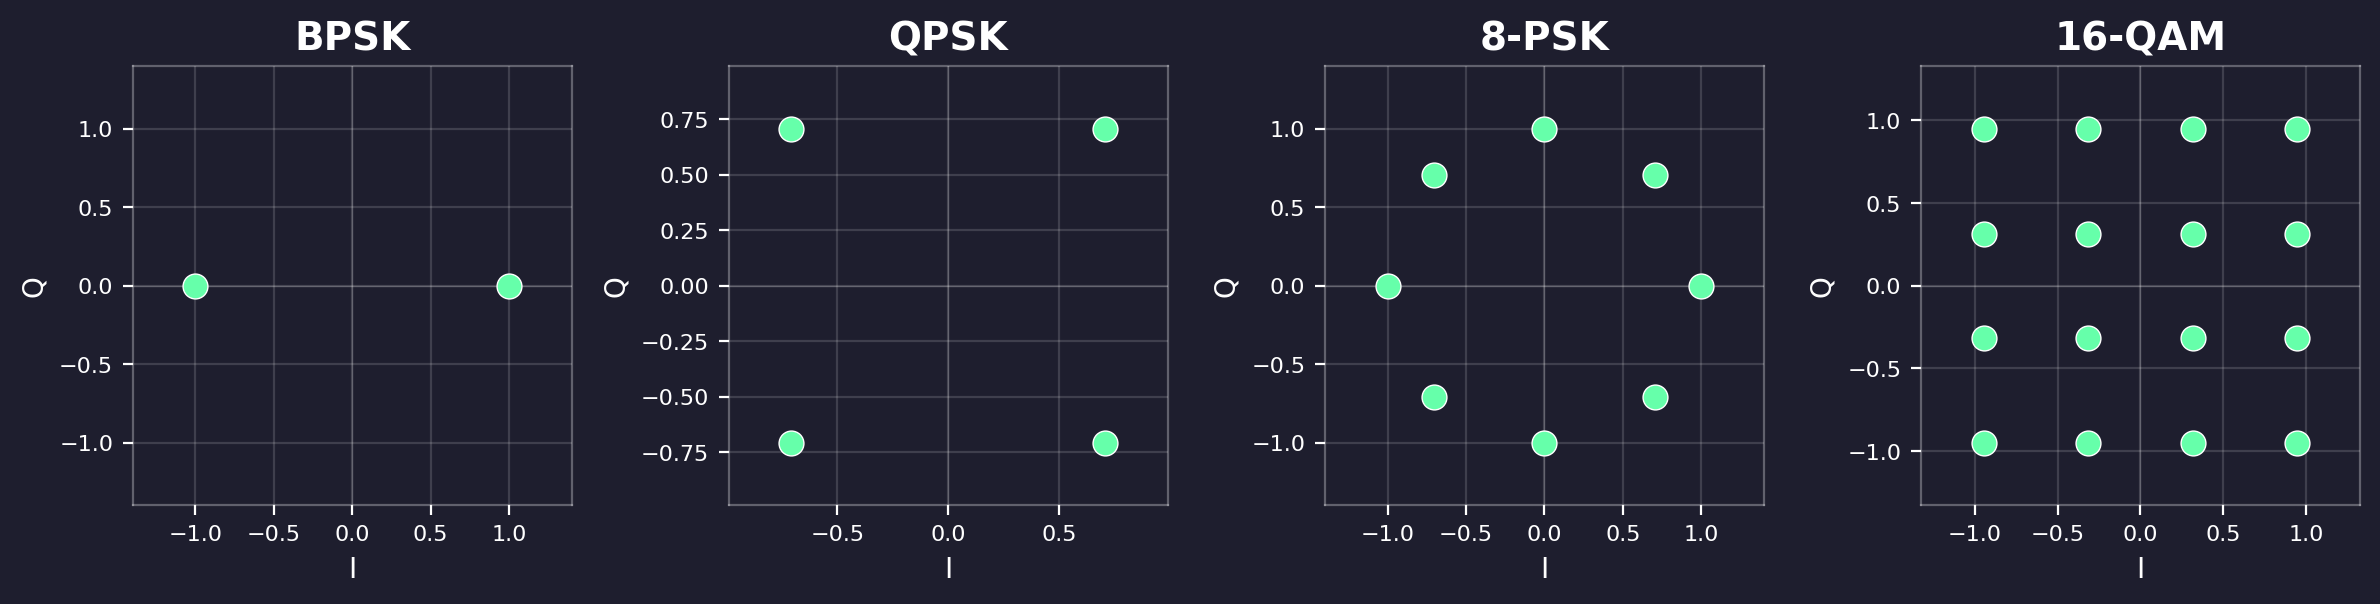
\includegraphics[width=0.9\textwidth]{constellations.png}
    \caption{The four constellations used in the demo.}
    \label{fig:const}
\end{figure}

\section{Code and GitHub}
\label{sec:availability}
Everything is here:

\begin{center}
\url{https://github.com/HowardWHSrun/E78FinalProject}
\end{center}

\noindent
Clone it, then use \texttt{README.md}. Layout: \texttt{main.py} at the root, code in \texttt{src/}, pictures in \texttt{figures/}, this PDF's \texttt{.tex} in \texttt{docs/}.

\section{How to run}
\texttt{pip install -r requirements.txt} from the repo root, then \texttt{python main.py}. Use \textbf{Connect Hardware} for the Pluto or \textbf{Simulation Mode} otherwise; press \textbf{Start}. Sliders change impairments; the \textbf{?} buttons explain each plot. \textbf{BER Sweep} runs automated SNR steps and overlays theory.

\begin{figure}[htbp]
    \centering
    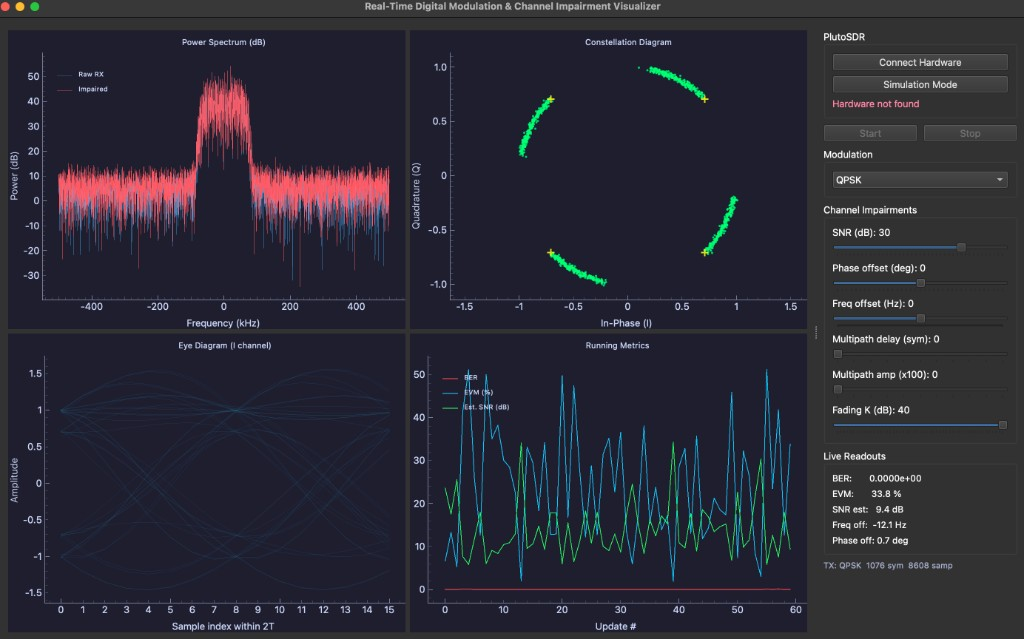
\includegraphics[width=0.85\textwidth]{gui_live.png}
    \caption{Live mode (example screenshot).}
    \label{fig:gui}
\end{figure}

\begin{figure}[htbp]
    \centering
    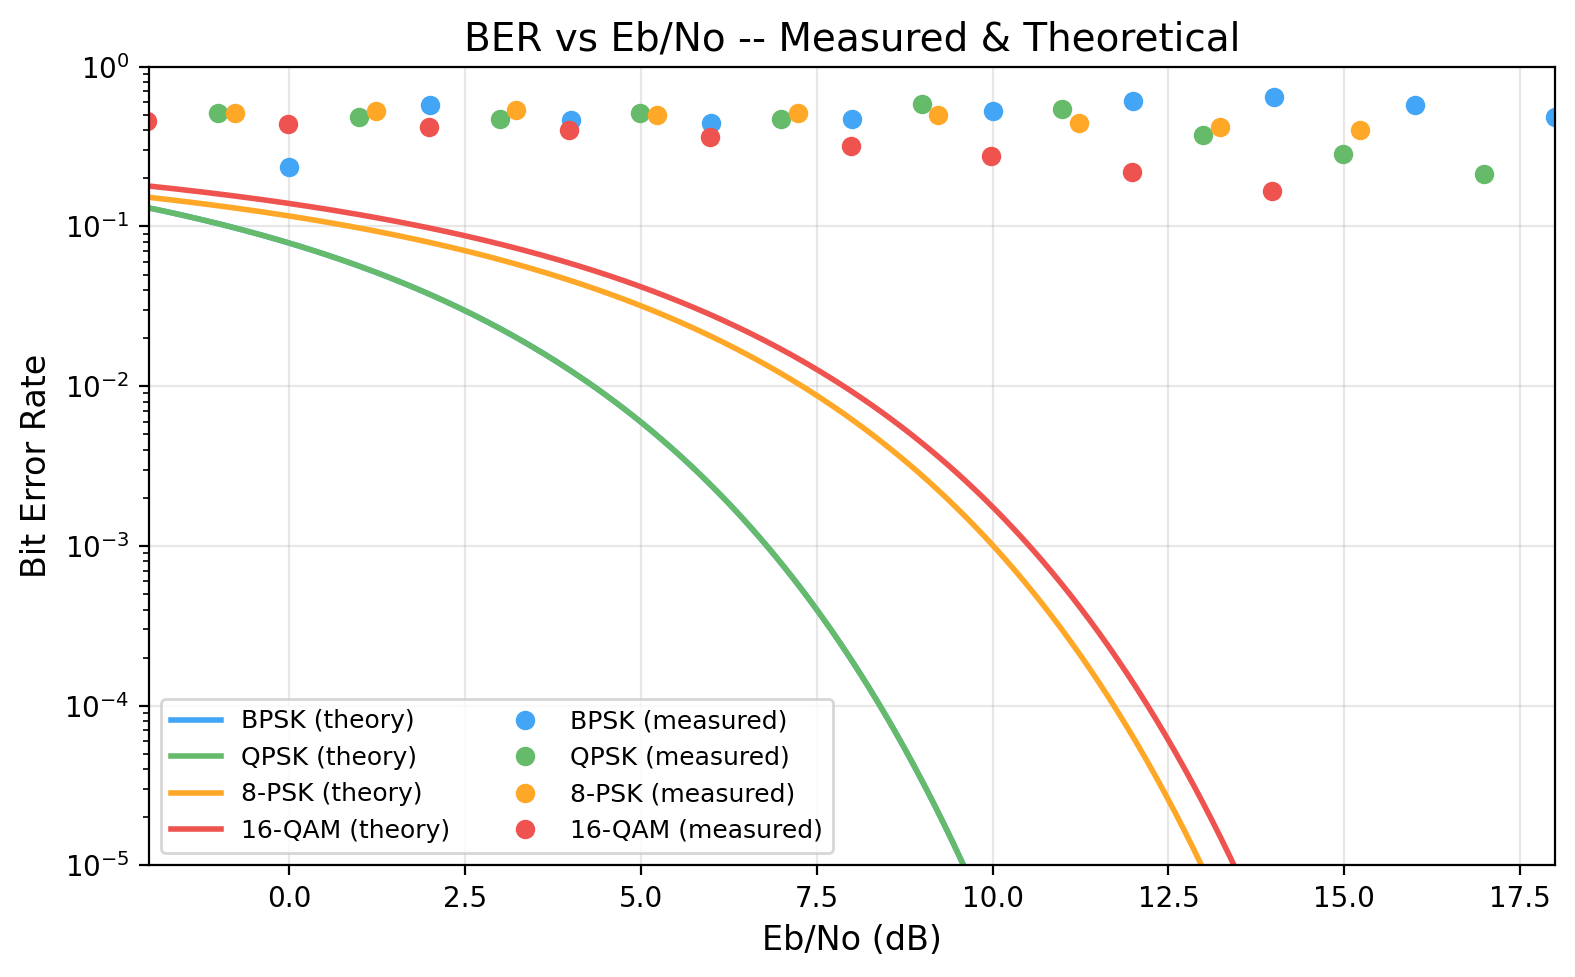
\includegraphics[width=0.85\textwidth]{ber_sweep.png}
    \caption{BER vs.\ $E_b/N_0$: measured points vs.\ theory.}
    \label{fig:ber}
\end{figure}

\section{Software (one table)}
The DSP runs in a background thread; the GUI reads shared results on a timer ($\sim$20~Hz) so the window stays responsive.

\begin{table}[htbp]
    \centering
    \small
    \begin{tabularx}{\linewidth}{@{}lX@{}}
        \toprule
        \textbf{File} & \textbf{What it does} \\
        \midrule
        \texttt{main.py} & Starts the app; adds \texttt{src/} to the path \\
        \texttt{src/gui.py} & PyQt6 UI, plots, BER sweep \\
        \texttt{src/dsp\_worker.py} & RX $\rightarrow$ impair $\rightarrow$ sync $\rightarrow$ demod \\
        \texttt{src/pluto\_interface.py} & Pluto or simulation \\
        \texttt{src/modulation.py}, \texttt{impairments.py}, \texttt{synchronization.py}, \texttt{ber\_sweep.py} & Modulation, channel, sync, sweep \\
        \bottomrule
    \end{tabularx}
\end{table}

\section{Results (brief)}
Measured BER vs.\ SNR tracks theory within about 1~dB under AWGN. Real hardware adds roughly 0.5--1~dB vs.\ simulation. Putting DSP in a worker thread and polling the GUI fixed lag we had when sending every buffer over Qt signals.

\section{Conclusion}
This project is a single-radio demo of modulation, impairments, and synchronization with live plots and a BER sweep. Extend it by adding schemes or impairment models in Python. See the GitHub link in Section~\ref{sec:availability}.

\begin{thebibliography}{9}
\bibitem{pluto} Analog Devices, ADALM-PLUTO documentation.\\\url{https://wiki.analog.com/university/tools/pluto}
\bibitem{proakis} J.\ G.\ Proakis and M.\ Salehi, \emph{Digital Communications}, McGraw-Hill.
\end{thebibliography}

\end{document}
